%%%%%%%%%%%%%%%%%%%%%%%%%%%%%%%%%%%%%%%%%%%%%%%%%%%%%%%%%%%%%%%%%%%%%
% PREAMBLE
%%%%%%%%%%%%%%%%%%%%%%%%%%%%%%%%%%%%%%%%%%%%%%%%%%%%%%%%%%%%%%%%%%%%%
%
% The following two commands will generate a PDF that follows all the requirements for submission
% and peer review.  Uncomment these commands to generate this output (and comment out the two lines below.)
%
% DOUBLE SPACE VERSION FOR SUBMISSION TO THE AMS
\documentclass[12pt]{article}
\usepackage{ametsoc}
%
% The following two commands will generate a single space, double column paper that closely
% matches an AMS journal page.  Uncomment these commands to generate this output (and comment
% out the two lines above. FOR AUTHOR USE ONLY. PAPERS SUBMITTED IN THIS FORMAT WILL BE RETURNED
% TO THE AUTHOR for submission with the correct formatting.
%
% TWO COLUMN JOURNAL PAGE LAYOUT FOR AUTHOR USE ONLY
%%%%\documentclass[10pt]{article}
%%%%\usepackage{ametsoc2col}
%
%%%%%%%%%%%%%%%%%%%%%%%%%%%%%%%%%%%%%%%%%%%%%%%%%%%%%%%%%%%%%%%%%%%%%
% ABSTRACT
%
% Enter your Abstract here
%%%%%%%%%%%%%%%%%%%%%%%%%%%%%%%%%%%%%%%%%%%%%%%%%%%%%%%%%%%%%%%%%%%%%
\newcommand{\myabstract}{
Direct measurements of rates of entrainment into and detrainment from cloud 
cores obtained from LES model cloud fields produce values twice as large as 
those produced from bulk conserved tracer budget calculations.  This difference 
can be explained by three effects: the presence of a shell of moist air around 
the cloud cores and drier air at the edge of the cloud core, correlations 
between entrainment rates and tracer values, and errors in the calculation of 
the bulk tracer budget.  Correlations between the vertical momentum and the 
entrainment rate create strong vertical momentum fluxes into the cloud core,
making the assumption that clouds entrain fluid with zero vertical momentum
incorrect.  Variability in the properties of the moist cloud shell has strong
impacts on entrainment values inferred from bulk tracer calculations.  These
results indicate the dynamics of the cloud shell should be included in 
parameterizations of cumulus clouds used in general circulation models.
}
%
\begin{document}
%
%%%%%%%%%%%%%%%%%%%%%%%%%%%%%%%%%%%%%%%%%%%%%%%%%%%%%%%%%%%%%%%%%%%%%
% TITLE
%
% Enter your TITLE here
%%%%%%%%%%%%%%%%%%%%%%%%%%%%%%%%%%%%%%%%%%%%%%%%%%%%%%%%%%%%%%%%%%%%%
\title{\textbf{\large{The influence of the cloud shell on bulk tracer 
measurements of LES cloud entrainment}}}
%
% Author names, with corresponding author information. 
% [Update and move the \thanks{...} block as appropriate.]
%
\author{\textsc{Jordan T Dawe}
				\thanks{\textit{Corresponding author address:} 
				Jordan T Dawe, Department of Earth and Ocean Sciences, 
                                University of British Columbia, 6339 Stores Road,
                                Vancouver, BC, V6T 1Z4, Canada.
				\newline{E-mail: jdawe@eos.ubc.ca}}\quad\textsc{and Philip H Austin}\\
\textit{\footnotesize{Department of Earth and Ocean Sciences, University of 
                      British Columbia, Vancouver, BC, Canada.}}
}
%
% Formatting done here...Authors should skip over this.  See above for abstract.
\ifthenelse{\boolean{dc}}
{
\twocolumn[
\begin{@twocolumnfalse}
\amstitle

% Start Abstract (Enter your Abstract above.  Do not enter any text here)
\begin{center}
\begin{minipage}{13.0cm}
\begin{abstract}
	\myabstract
	\newline
	\begin{center}
		\rule{38mm}{0.2mm}
	\end{center}
\end{abstract}
\end{minipage}
\end{center}
\end{@twocolumnfalse}
]
}
{
\amstitle
\begin{abstract}
\myabstract
\end{abstract}
}
%%%%%%%%%%%%%%%%%%%%%%%%%%%%%%%%%%%%%%%%%%%%%%%%%%%%%%%%%%%%%%%%%%%%%
% MAIN BODY OF PAPER
%%%%%%%%%%%%%%%%%%%%%%%%%%%%%%%%%%%%%%%%%%%%%%%%%%%%%%%%%%%%%%%%%%%%%
\section{Introduction}

The rate at which air is entrained into and detrained from cumulus clouds 
affects cloud properties, cloud top height, and vertical transports of heat 
and moisture.  Proper simulation of these subgrid-scale effects in General 
Circulation Models (GCM) depends on the accurate parameterization of 
entrainment of environmental tracer properties into the clouds and detrainment 
of cloud properties into the environment 
\citep{Bechtold2008, De_Rooy2010}.  

Entrainment and detrainment rates impact GCM parameterizations in serveral ways.
First, profiles of cloud vertical mass flux are usualy calculated from 
parameterizated entrainment values using the continuity equation for a 
simple entraining plume:
\begin{equation}
   \label{eq:continuity}
   \rho \frac{\partial a}{\partial t} 
   + \frac{\partial M_{core}}{\partial z} = E - D.
\end{equation}
The point where this mass flux profile goes to zero then defines the location 
of cloud top.  This mass flux profile is combined with the entrainment rate 
of environmental air into the cloud to calculate vertical profiles of moisture
and temperature in the cloud, and these profiles are then used to calculate 
the moistening of the environment by detrainment of fluid from the clouds.
Precipitation rates are also generated from the mass flux and tracer profiles 
produced from the entrainment and detrainment profiles.  The wide range of
effects that the entrainment and detrainment have make entrainment rate one of
the strongest controls on the climate sensitivity of GCMs 
\citep{Stainforth2005, Rougier2009}.

Large Eddy Simulation (LES) is the primary tool used to study cloud entrainment
and detrainment rates.  LES mass entrainment and detrainment rates are typically
calculated using budgets of bulk conserved tracer variables to infer the amount
of fluid exchange between the clouds and the surrounding air.  These rates are
then used in simple entraining plume parameterizations to evaluate sub-grid 
scale cloud transports.  \cite{Siebesma1995} derive the following equations for
entrainment and detrainment of mass from a cloud core plume, where cloud core 
is defined as regions having condensed liquid water, positive buoyancy, and 
upward vertical velocity:
\begin{equation}
  \label{eq:siebesma_entrainment}
    E_{\phi S}(\phi_{core} - \phi_{env}) = - M_{core} \frac{\partial \phi_{core}}{\partial z}
        - \frac{\partial \rho a \overline{w' \phi'}^{core}}{\partial z}
        - \rho a \frac{\partial \phi_{core}}{\partial t}
        + a \rho \left(\frac{\partial \bar{\phi}}{\partial t}\right)_{forcing}
\end{equation}
and
\begin{equation}
  \label{eq:siebesma_detrainment}
    D_{\phi S}(\phi_{core} - \phi_{env}) = - M_{core} \frac{\partial \phi_{env}}{\partial z}
        + \frac{\partial \rho (1 - a) \overline{w' \phi'}^{env}}{\partial z}
        + \rho (1-a) \frac{\partial \phi_{env}}{\partial t}
     - \rho (1-a) \left(\frac{\partial \bar{\phi}}{\partial t}\right)_{forcing}
\end{equation}
Here $\phi$ represents any conserved bulk tracer, such as the total specific 
humidity $q_t$ (kg water kg$^{-1}$ moist air) or the liquid-water moist static 
energy $h$ (J kg$^{-1}$), $a$ is the fractional cloud core area, $\rho$ is the
density of the air in kg m$^{-3}$, $M_c$ is vertical cloud core mass flux 
(kg m$^{-2}$ s$^{-1}$), $w$ is vertical velocity (m s$^{-1}$), $env$ and 
$core$ sub-and super-scripts denote horizontally averaged values conditionally
sampled in the cloud environment and core, $forcing$ refers to tracer sources 
and sinks, such as radiation or subsidence, not included in the other terms,
primed values represent anomalies relative to the horizontal mean, overbars
represent horizontal averaging, and $E_{\phi S}(z)$ and $D_{\phi S}(z)$ are the 
total mass entrainment into and detrainment from the cloud core inferred from 
the bulk tracer budget, in kg s$^{-1}$ m$^{-3}$.  We use the $S$ subscript
to differentiate $E$ and $D$ calculated via the Siebesma bulk tracer budget 
method from other measures of mass exchanges, and we shall refer to values calculed by this method as ``Siebesma tracer budget" entrainment and 
detrainment.

Alternatively, entrainment and detrainment of mass can be calculated directly
from the LES velocity and tracer fields.  \cite{Romps2010} recently presented a 
technique to measure local (grid scale) mass entrainment $e(x,y,z)$ and
detrainment $d(x,y,z)$.  Summing these point measurements horizontally gives 
$E_d(z)$ and $D_d(z)$, the total mass entrained into and detrained from the
cloud core field in kg s$^{-1}$ m$^{-3}$, where the $d$ subscript indicates 
these quantities were calculated directly from the model velocity and tracer
fields.  His equation (2) is:
\begin{equation}
  \label{eq:romps_e_minus_d}
  e - d = \frac{\partial}{\partial t}(\mathcal{A}\rho) 
        + \nabla \cdot (\rho \mathbf{u} \mathcal{A}) 
\end{equation}
Here $e$ and $d$ are the local entrainment and detrainment of mass through the 
cloud core surface in kg s$^{-1}$ m$^{-3}$, $\mathbf{u}$ is the velocity of the 
air in m s$^{-1}$, and $\mathcal{A}$ is the ``activity" of the fluid, where 
$\mathcal{A}$ is one at cloud core points and zero otherwise.  The values of 
$e - d$ are averaged over the time that a grid cell experiences mass fluxes
between an active and an inactive point, then positive $e-d$ values are
considered to be purely $e$, and negative values, $d$.  We shall refer in the text to entrainment and detrainment values calculated by this method as ``direct"
$E$ and $D$.

Romps found that direct calculates of entrainment and detrainment mass fluxes
produced values roughly twice as large as Siebesma tracer budget calculations.  Romps attributed this difference to the Siebesma tracer budget calculation assumption that fluid exchanged between clouds and environment has the mean
properties of the cloud or environment, respectively.  Recent studies of the
dense, descending shell of moist air that forms around trade-wind cumulus clouds
\citep{Heus2008, Wang2010} suggest that the cloud shell properties are quite
different than the core or environment properties, bolstering Romps' hypothesis.
Since fluid exchanges between clouds and environment must pass through this
shell, it is likely that it plays an important role in entrainment and
detrainment dynamics.

Here we examine the sources of the discrepancy in entrainment and detrainment
values calculated via bulk tracer budgets and directly from model fluxes.  We
show that the discrepancy is explained by three effects: the presence of the
shell of moist air around the cloud cores and drier air at the edge of the 
cloud core, correlations between local entrainment rates and tracer values 
which enhance tracer fluxes between the clouds and the environment, and errors 
in the calculation of the bulk tracer budget.  We derive a relation to convert 
the ``direct" entrainment flux values into ``Siebesma tracer budget" values 
suitable for use in one-dimensional simple entraining plume cloud
parameterizations, and then use this to evaluate the impact of the shell on 
bulk tracer entrainment and detrainment rates of humidity and vertical 
velocity.  Finally, we examine the dynamics that drives the strong correlations
we find between entrainment rate, humidity, and vertical velocity.

%===================================================

\section{Model description}

All LES calculations in this paper were made using the System for Atmospheric 
Modeling \citep[SAM;][]{Khairoutdinov2003}.  Two model runs were performed, 
configured as standard Global Energy and Water Cycle Experiment (GEWEX) 
Cloud System Studies \citep[GCSS;][]{Randall2003} experiments: a Barbados 
Oceanographic and Meteorological Experiment \citep[BOMEX;][]{Siebesma2003} run,
and an Atmospheric Radiation Measurement Study \citep[ARM;][]{Brown2002} run. 
The BOMEX run was performed on a 6.4 km x 6.4 km horizontal x 3.2 km vertical 
domain with 25 meter grid size in all directions for 6 hours, and the first 
three hours of simulation were discarded. The ARM run was performed on a 
7.68 km x 7.68 km x 4.5 km domain with 30 meter grid size.  Precipitation was 
disabled in both runs.

We have implemented the entrainment calculation scheme of \cite{Romps2010} in 
SAM, allowing us to calculate the mass of air entrained into and detrained from
cloud core directly from model $\rho$, $\mathbf{u}$, and $\mathcal{A}$.  
\citet[eq. 4]{Romps2010} also presents a method for calculating local 
entrainment and detrainment rates for any model bulk variable in the same
framework as (\ref{eq:romps_e_minus_d}), but neglects forcing and diffusion
terms.  These terms are significant for quantities like vertical momentum, so 
we modify Romps's equation to include their effects:
\begin{equation}
  \label{eq:romps_ephi_minus_dphi}
  e\phi - d\phi = \frac{\partial}{\partial t}(\phi \mathcal{A} \rho) 
                + \nabla \cdot (\phi \rho \mathbf{u} \mathcal{A})
                - \rho \mathcal{A}S_\phi
\end{equation}
where $S_\phi$ is any non-advective source or sink term for $\phi$, such as 
precipitation for $q_t$ or radiation for $h$, in units of $[\phi]$ s$^{-1}$.  

As with equation (\ref{eq:romps_e_minus_d}), $e\phi$ and $d\phi$ must be 
horizontally summed to give the total tracer entrained into or detrained out 
of the cloud ensemble, but since $\phi$ can be negative, it is possible for 
entrainment to reduce and for detrainment to increase the tracer quantity 
in the cloud core.  To accomodate this effect, if the average value of $\phi$ 
is positive over the time that a grid cell experiences mass fluxes between an 
active and an inactive point, then positive $e\phi-d\phi$ values are 
considered to be purely $(e\phi)(x,y,z)$, and negative values, $(d\phi)(x,y,z)$. 
However, if the average of $\phi$ is negative, then positive $e\phi-d\phi$ 
values are considered to be purely $(d\phi)(x,y,z)$, and negative values, 
$(e\phi)(x,y,z)$.  Horizontal summation of $(e\phi)$ and $(d\phi)$ then 
gives $(E\phi)_d(z)$ and $(D\phi)_d(z)$, the total entrainment and detrainment 
of tracer for the cloud ensemble in $[\phi]$ kg s$^{-1}$ m$^{-3}$, where the 
$d$ subscript indicates these quantities were calculated directly from the 
model velocity and tracer fields.

%===================================================

\section{Relationship Between Direct and Bulk Tracer Budget Entrainment}

\cite{Romps2010} established that directly measured mass entrainment and 
detrainment is roughly twice the size of values calculated via bulk 
tracer budgets.  This is a worrying difference, but might not have important
effects on GCM cloud parameterizations if this ratio is constant.  
However, examination of the ratios of Siebesma tracer budget mass entrainment 
and detrainment calculated via a total specific water budget ($E_qS$, $D_qS$) 
to the directly calculated values ($E_d$, $D_d$) over the diurnal cycle of an 
ARM LES reveals significant changes over the course of the day 
(Fig. \ref{fig:entrainment_ratio_variability}).  Bulk tracer and direct 
measurements of $E$ and $D$ have differing dynamics which may need to be 
included in parameterizations.  In this section we examine the sources of 
disagreement between direct and Siebesma tracer budget estimates of mass entrainment into and detrainment from the cloud core.

%---------------------------------------------------

\subsection{$E$ and $D$ Cloud Shell Correction}

Romps attributed the differences between ($E_{\phi S}$, $D_{\phi S}$) and 
($E_d$, $D_d$) to the assumption made by \cite{Siebesma1995} that fluid 
entrained or detrained has the properties of the mean environment or 
cloud core, respectively.  However, if we examine the specific 
humidity of the fluid at the ``cloud core edge" (cloud core model grid 
cells that are nearest-neighbor adjacent to non-core cells), which 
presumably is the fluid being detrained, we see it is drier than the mean 
core (Fig. \ref{fig:Shell_correction}a).  Similarily, the fluid just 
outside the cloud core in the ``cloud core shell" (non-core model 
grid cells that are nearest-neighbor adjacent to core cells) which is 
available for entrainment is moister than the mean environment.
  
Here we derive a correction to equations (\ref{eq:siebesma_entrainment}) and 
(\ref{eq:siebesma_detrainment}) to account for the presence of the moist cloud 
shell and dry cloud edge, allowing us to transform ($E_d, D_d$) values into 
equivalent Siebesma tracer budget values ($E_{\phi}, D_{\phi}$).  We start
our derivation by modifying equations (5.1) from
\cite{Siebesma1995}:
\begin{eqnarray}
  \label{eq:entrainment_derivation_1}
    \rho \frac{\partial a \phi_{core}}{\partial t} 
    = - \frac{\partial M_{core} \phi_{core}}{\partial z} 
    + E_d \phi_E - D_d \phi_D
    - \frac{\partial \rho a \overline{w' \phi'}^{core}}{\partial z} 
    + a \rho \left(\frac{\partial \bar{\phi}}{\partial t}\right)_{forcing}
\end{eqnarray}
\begin{eqnarray}
  \label{eq:detrainment_derivation_1}
    \rho \frac{\partial (1 - a) \phi_{env}}{\partial t}
    = \frac{\partial M_{core} \phi_{env}}{\partial z} 
    - E_d \phi_E + D_d \phi_D
    - \frac{\partial \rho (1 - a) \overline{w' \phi'}^{env}}{\partial z} 
    + \rho (1 - a) \left(\frac{\partial \bar{\phi}}{\partial t}\right)_{forcing}.
\end{eqnarray}
Here we have replaced $\phi_{env}$ in the entrainment term with $\phi_E$ and 
$\phi_{core}$ in the detrainment term with $\phi_D$, where $\phi_E$ and $\phi_D$
are the tracer values of the air being entrained and detrained, respectively.

Next we substitute equation (\ref{eq:continuity}), the continuity equation 
for a cloud plume, into (\ref{eq:entrainment_derivation_1}) 
and (\ref{eq:detrainment_derivation_1}) allowing us to write
\begin{eqnarray}
  \label{eq:entrainment_derivation_2}
    E_d (\phi_{core} - \phi_E) - D_d (\phi_{core} - \phi_D)
    = M_{core} \frac{\partial \phi_{core}}{\partial z}
    + \frac{\partial \rho a \overline{w' \phi'}^{core}}{\partial z} 
    + \rho a \frac{\partial \phi_{core}}{\partial t}
    - a \rho \left(\frac{\partial \bar{\phi}}{\partial t}\right)_{forcing}
\end{eqnarray}
\begin{eqnarray}
  \label{eq:detrainment_derivation_2}
    D_d (\phi_D - \phi_{env}) - E_d (\phi_E - \phi_{env})
    = - M_c \frac{\partial \phi_{env}}{\partial z}
    + \frac{\partial \rho (1 - a) \overline{w' \phi'}^{env}}{\partial z} 
    + \rho (1 - a) \frac{\partial \phi_{env}}{\partial t}
    - \rho (1 - a) \left(\frac{\partial \bar{\phi}}{\partial t}\right)_{forcing}.
\end{eqnarray}

We then substitute in equations (\ref{eq:siebesma_entrainment}) and 
(\ref{eq:siebesma_detrainment}) for the bulk tracer tendency terms and 
rearrange to get:
\begin{equation}
  \label{eq:corrected_entrainment}
    E_{\phi T} = E_d 
             - \left[E_d\frac{(\phi_E - \phi_{env})}{(\phi_{core} - \phi_{env})}
                   + D_d\frac{(\phi_{core} - \phi_D)}{(\phi_{core} - \phi_{env})}\right]
\end{equation}
\begin{equation}
  \label{eq:corrected_detrainment}
    D_{\phi T} = D_d
             - \left[E_d\frac{(\phi_E - \phi_{env})}{(\phi_{core} - \phi_{env})}
                   + D_d\frac{(\phi_{core} - \phi_D)}{(\phi_{core} - \phi_{env})}\right].
\end{equation}
Thus, to convert from ($E_d$,$D_d$) to ($E_{\phi T}$, $D_{\phi T}$), both 
$E_d$ and $D_d$ must be reduced by $E_d A + D_d B$, where
$A = (\phi_E - \phi_{env})/(\phi_{core} - \phi_{env})$ and
$B = (\phi_{core} - \phi_D)/(\phi_{core} - \phi_{env})$.  Here we have added 
the $T$ subscript to the $E_{\phi T}$ and $D_{\phi T}$ terms to denote these
values are equivalent to Siebesma tracer budget values, but have been 
calculated by transforming the direct entrainment and detrainment values.  
We shall refer to these values as ``transformed" entrainment and detrainment.  

Alternatively, we can solve for $E_d$ and $D_d$, arriving at
\begin{equation}
  \label{eq:corrected_entrainment2}
    E_{d T} = E_{\phi S} 
        + \left[E_{\phi S}\frac{(\phi_E - \phi_{env})}{(\phi_D - \phi_E)} 
              + D_{\phi S}\frac{(\phi_{core} - \phi_D)}{(\phi_D - \phi_E)}\right].
\end{equation}
\begin{equation}
  \label{eq:corrected_detrainment2}
    D_{d T} = D_{\phi S} 
        + \left[E_{\phi S}\frac{(\phi_E - \phi_{env})}{(\phi_D - \phi_E)}
              + D_{\phi S}\frac{(\phi_{core} - \phi_D)}{(\phi_D - \phi_E)}\right].
\end{equation}
In this case, to convert from ($E_{\phi S}$, $D_{\phi S}$) to 
($E_{dT}$, $D_{dT}$), both $E_{\phi S}$ and $D_{\phi S}$ must be increased by 
$E_{\phi S} a + D_{\phi S} b$, where 
$a = (\phi_E - \phi_{env})/(\phi_{core} - \phi_{env})$ and 
$b = (\phi_{core} - \phi_D)/(\phi_{core} - \phi_{env})$.  Note that under both these transformations $E_d-D_d = E_{\phi}-D_{\phi}$, preserving mass continuity,
and furthermore, $E_d A + D_d B = E_{\phi} a + D_{\phi} b$.

We now have relationships allowing us to transform the biased Siebesma tracer
budget $E_{\phi S}$ and $D_{\phi S}$  values into unbiased $E_{dT}$ and $D_{dT}$
values, and vice versa.  However, since our main concern is with improving GCM
cloud parametertizations, we will focus on equations 
(\ref{eq:corrected_entrainment}) and (\ref{eq:corrected_detrainment}) which 
convert the directly calculated entrainment and detrainment into values 
more suitable for simple entraining plume parameterizations of cloud fields.

Comparison of $E_{q S}$ and $D_{q S}$ ($E_{\phi S}$ and $D_{\phi S}$ inferred
using total specific moisture $q_t$ as the bulk tracer) with $E_d$ and $D_d$
shows the direct entrainment and detrainment values are significantly larger 
than the Siebesma tracer budget values (Figure \ref{fig:Shell_correction}, 
b and c).  Using equations (\ref{eq:corrected_entrainment}) and 
(\ref{eq:corrected_detrainment}) to calculate $E_{q T}$ and $D_{q T}$ from 
using $q_E = q_{edge}$ and $q_D = q_{shell}$ results in values quite close to 
the Siebesma tracer budget values.  Relative to the Siebema tracer budget
values, the transformed $E_{q T}$ and $D_{q T}$ values are still too large 
near cloud base.  However, the transformation does duplicate the negative 
$D_{q S}$ values near cloud base that are typically produced by bulk tracer calculations.

%-------------------------------------------------------------------------

\subsection{Entrainment/Tracer Correlations}

We can partially explain the difference between the transformed mass 
entrainment/detrainment values and the Siebesma tracer budget values as 
being the result of correlations between the local entrainment/detrainment 
rates and the local tracer properties in the shell and edge.  Using the 
mean shell and edge values of tracers to transform the direct entrainment 
and detrainment assumes that any fluid parcel in the shell or edge is 
equally likely to be entrained or detrained.  In reality, mixing relatively 
dry air into the cloud core is more likely to cause evaporation, which will 
drive detrainment, while mixing relatively moist air is more likely to 
produce a saturated fluid mixture, resulting in entrainment.

If there are correlations between entrainment/detrainment and the local 
fluid properties, this will result in the effective tracer value being 
entrained into or detrained from the cloud core being different than the 
mean tracer value in the shell or edge.  We can directly calculate the 
effective tracer value at which entrainment occurs by taking the total 
tracer entrainment $(E\phi)_d$ calculated via equation 
(\ref{eq:romps_ephi_minus_dphi}) and dividing it by the total mass
entrainment $E_d$ so that $\phi_{entrain} = (E\phi)_d / E_d$.  Similarily, 
the effective tracer value at which detrainment occurs van be found from  
$\phi_{detrain} = (D\phi)_d / D_d$.  Examination of these values from the 
BOMEX simulation using $q_t$ for $\phi$ shows $q_{entrain}$ is moister than 
$q_{shell}$ (Figure \ref{fig:Reynolds_correction}a), indicating entrainment
occurs preferentially at the moistest parts of the shell.  Conversely, 
there is little difference between between $q_{detrain}$ and $q_{edge}$,
indicating no significant correlation between detrainment and the moisture
present in the cloud core edge.

Using $q_{entrain}$ and $q_{detrain}$ to transform $E_d$ and $D_d$ values 
results in smaller $E_{q T}$ and $D_{q T}$ values than utilizing the mean 
shell and edge properties (Fig. \ref{fig:Reynolds_correction}, b and c).  
Unfortunately, this actually reduces the agreement between transformed 
$E_{q T}$ and $D_{q T}$ values and the Siebesma tracer budget values 
$E_{q S}$ and $D_{q S}$ compared to using the shell and edge properties.
 However, it also reduces the large entrainment and detrainment values near 
cloud base, which improves the overall shape of the fluxes.  Still, 
$E_{q T}$ calculated using $q_E = q_{entrain}$ and $q_D = q_{detrain}$ is 
about half the magnitude of the Siebesma tracer budget entrainment value.

%------------------------------------------------------------------------------

\subsection{Tracer Budget Errors}

The final possible source of differences between the Siebesma tracer 
budget entrainment and detrainment and the transformed values is biases
in the tracer budget calculation (equations (\ref{eq:siebesma_entrainment})
and (\ref{eq:siebesma_detrainment})).  The Siebesma tracer budget calculates 
vertical advection of tracer properties by taking derivatives of mean 
vertical tracer profiles, along with averaged vertical Reynolds fluxes.  
There is no guarantee this estimate of vertical advection will exactly 
agree with the fully three dimensional MPDATA advection algorithm used by 
SAM.  In fact, the differences in the numerics of these calculations 
likely insures the results, while similar, will not be exactly the 
same.  Furthermore, the Siebesma calculation neglects tracer diffussion.  
These effects are likely small, but the exact amount of error they 
induce is difficult to evaluate.

\cite{Romps2010} presents an alternate method of calculating bulk tracer
budget entrainment and detrainment values (Romps' equations (11) and (12))
using the direct mass and $\phi$ entrainment/detrainment rates and mean 
profiles of $\phi_{core}$ and $\phi_{env}$ to calculate vertical advection 
and time tendency budgets:
\begin{equation}
  \label{eq:romps_bulk_entrainment}
    E_{\phi R}(\phi_{core} - \phi_{env}) = \phi_{core}(E_d-D_d) - ((E\phi)_d - (D\phi)_d)
\end{equation}
\begin{equation}
  \label{eq:romps_bulk_detrainment}
    D_{\phi R}(\phi_{core} - \phi_{env}) = \phi_{env}(E_d-D_d) - ((E\phi)_d - (D\phi)_d)
\end{equation}
Here the $R$ subscript indicates that $E$ and $D$ have been calculated via 
the Romps bulk tracer budget method, and we shall refer to values calculed 
by this method as ``Romps tracer budget" $E$ and $D$.

The Romps tracer budget equations are exactly analagous with the Siebesma 
tracer budget equations.  Using equation (\ref{eq:continuity}) it is easy 
to show that
\begin{equation}
    \phi_{core}(E_d - D_d) =
    \phi_{core} \left(\rho \frac{\partial a}{\partial t}
                    + \frac{\partial M_{core}}{\partial z}\right).
\end{equation}
Similarly, the tracer continuity equation can be used to show that
\begin{equation}
    (E\phi)_d - (D\phi)_d) = 
     \rho \frac{\partial (a \phi_{core})}{\partial t}
   + \frac{\partial (M_{core} \phi_{core})}{\partial z}
   + \frac{\partial \rho a \overline{w' \phi'}^{core}}{\partial z}
   - a \rho \left(\frac{\partial \bar{\phi}}{\partial t}\right)_{forcing}.
\end{equation}
Subtracting $(E\phi)_d - (D\phi)_d)$ from $\phi_{core}(E_d - D_d)$ then 
results in the budget terms of equation (\ref{eq:siebesma_entrainment}).

Note that by substituting $(E \phi)_d = E_d \phi_E$ and 
$(D\phi)_d = D_d \phi_D$ into (\ref{eq:romps_bulk_entrainment}) and 
(\ref{eq:romps_bulk_detrainment}), we can quickly recover the 
equations to transform direct entrainment/detrainment values into 
equivalent tracer budget values (equations (\ref{eq:corrected_entrainment}) 
and (\ref{eq:corrected_detrainment})).  This equivalence between equations 
(\ref{eq:corrected_entrainment}), (\ref{eq:corrected_detrainment}) and 
equations (\ref{eq:romps_bulk_entrainment}), (\ref{eq:romps_bulk_detrainment})
means the Romps tracer budget formulation agrees exactly with the result of 
using $q_{entrain}$ and $q_{detrain}$ values to transform the direct 
entrainment and detrainment into equivalent bulk tracer values.  

Comparing the Romps and Siebesma $q_{core}(E_d - D_d)$ values (Fig. \ref{fig:numerical_error}a) shows the Romps value is has a significantly smaller 
magnitude than the Siebesma value.  The $((Eq_t)_d - (Dq_t)_d)$ values 
(Fig. \ref{fig:numerical_error}b) shows the same smaller magnitude for
the Romps value compared to the Siebesma value.  The reason for this can 
be seen by comparing these calculations with a version of the direct 
entrainment calculation done without any time averaging of the fluxes.  
Without time averaging, the direct entrainment and detrainment values are 
far too large, but the continuity equation (equation (\ref{eq:continuity})) ensures that $E-D$ is the same size.  Indeed, the unaveraged 
$\phi_{core}(E_d - D_d)$ value agrees almost exactly with the Siebesma 
tracer budget value $\phi_{core}(E_{qS} - D_{qS})$.  Due to the time 
averaging of the direct entrainment and detrainment, the direct 
calculation always has a pool of ``activity flux" which has not yet been 
assigned to either $E_d$ or $D_d$.  This reduces both $E_d$ and $D_d$ by 
roughly the same proportion, causing $E_d-D_d$ to be smaller than the 
unaveraged and Siebesma $E_{qS}-D_{qS}$ values.

However, despite the large differences between the $q_{core}(E_d - D_d)$
and $((Eq_t)_d - (Dq_t)_d)$ direct calculation values with and without
time averaging, the net tracer budget that results from the differences 
between these terms (Fig. \ref{fig:numerical_error}c) agrees remarkably 
well with the unaveraged calculation.  Conversely, the Siebesma tracer 
budget that results is much larger than the Romps tracer budget, despite 
the close agreement between the Siebesma and Romps tracer budget 
$q_{core}(E_d - D_d)$ and $((Eq_t)_d - (Dq_t)_d)$ values.  This difference
between the tracer budgets calculated by the Siebesma and Romps methods is 
the source of the remaining differences between the direct and Siebesma
entrainment and detrainment calculations.

Evaluating which of the two budget calculations is more accurate is difficult.
We discussed the possible problems in the Siebesma tracer budget
calculation related to neglect of tracer diffusion and the simplified method 
used to calculating vertical advection.  The Romps tracer budget, on the 
other hand, requires taking the difference of $q_{core}(E_d - D_d)$
and $((Eq_t)_d - (Dq_t)_d)$, terms which have nearly the same magnitude.  
Because of this, small relative errors in these terms can result in large 
relative errors when their difference is taken.  Consider, for example, the 
tiny difference between the unaveraged direct and Siebesma 
$((Eq_t)_d - (Dq_t)_d)$ values (Fig. \ref{fig:numerical_error}b).  Although
the Siebesma tracer budget $((Eq_t)_d - (Dq_t)_d)$ is only slightly different
than the unaveraged direct flux value, this results in a relatively large 
difference between the unaveraged direct tracer budget and Siebesma tracer
budgets (Fig. \ref{fig:numerical_error}c).  Both of the calculation methods
thus have possible sources of error.

%==============================================================================

\section{$E_q$, $E_h$ and $E_w$ Differences}

Equations (\ref{eq:corrected_entrainment}) or (\ref{eq:corrected_detrainment}) 
imply that the Siebesma tracer budget method will measure different entrainment
and detrainment values for fluid properties with differing values of 
$A = (\phi_E - \phi_{env})/(\phi_{core} - \phi_{env})$ and
$B = (\phi_{core} - \phi_D)/(\phi_{core} - \phi_{env})$.  With this in mind 
we compare transformed $E_{\phi T}$ and $D_{\phi T}$ values produced by liquid
water moist static energy $h$ and vertical velocity $w$.

Liquid water moist static energy shows a similar relative distribution of 
core, edge, shell, environment, entrain and detrain properties when compared 
to $q_t$, indicating a tight coupling between these variables in the cloud
dynamics.  Because these properties are so tightly coupled, the transformed 
$E_{hT}$ and $D_{hT}$ values are nearly identical to the $E_{qT}$ and 
$D_{qT}$ (not shown).

Vertical velocity shows very different relative profiles compared to
$q_t$ and $h$ (Fig. \ref{fig:Reynolds_correction_w}a).  There is a much wider spread in the $w$ values, with the shell having nearly zero vertical velocity 
and the edge being halfway between the core and the environment.  $w_{detrain}$ 
is slightly larger than the value of $w$ in the edge, while $w_{entrain}$ is 
much larger than $w$ in the shell, becoming roughly the same value as 
$w_{edge}$.  Since $w_{entrain}$ and $w_{detrain}$ are both larger than 
$w_{shell}$ and $w_{edge}$ this implies that the air that is moving upward 
the fastest is both preferentially entrained and detrained.  Furthermore, 
the large difference between $w_{entrain}$ and $w_{shell}$ indicates that 
local $w$ is strongly correlated with local entrainment.  These effective
entrainment and detrainment $w$ values produce $E_{wT}$ and $D_{wT}$ that 
are quite different than the transformed entrainment and detrainment produced 
by $q_t$ and $h$ (Fig. \ref{fig:Reynolds_correction_w}b and c); 
$E_{wT}$ is negative over the whole of the cloud field, and $D_{wT}$ is half 
the magnitude of $D_{qT}$ over much of the cloud layer.

Finally, we examine the temporal variability of 
$A = (\phi_E - \phi_{env})/(\phi_{core} - \phi_{env})$ and
$B = (\phi_{core} - \phi_D)/(\phi_{core} - \phi_{env})$ from the transformation
equations (\ref{eq:corrected_entrainment}) and (\ref{eq:corrected_detrainment})
in the ARM model run.  These quantities show strong changes over the ARM diurnal
cycle (Figure \ref{fig:shell_variability}).  Near cloud base and within the
inversion, $A$ is nearly one while $B$ is nearly zero.  As the clouds mix 
into the inversion over the course of the day, the values calculated using 
$q_t$ evolve until at mid-cloud layer, $A$ has values near 0.6 and $B$ near 
0.2.  When calculated for $w$ on the other hand, $A$ reaches a value around 
0.5 and $B$ goes to 0.6.  Performing this calculation with fixed values of 
$(\phi_{core} - \phi_{env})$, to remove changes due to movement of the mean
environment and core profiles, shows similar results.  Changes in the 
properties of the entraining and detraining fluid clearly are active in
determining the magnitude of the rates at which properties entrain and detrain.

%-------------------------------------------------------------------------

\section{Causes of $e$, $q$, and $w$ Correlations}

The source of the correlations between entrainment, $q_t$, $h$, and $w$ can 
be seen by comparing instantaneous snapshots of the model values of mass entrainment $e$, moisture entrainment $e{q_t}$, and vertical velocity 
entrainment $e{w}$.  Since the \cite{Romps2010} method of calculating 
$e$ and $d$ requires taking time averages, it is unsuitable for calculating instantaneous entrainment fields.  Instead, we use an alternative method that 
we have devised that substitutes spatial interpolation for time averaging 
\citep{Dawe2011}.  This alternative method results in slightly smaller values 
of $e$ and $d$ than those produced by Romps' method, but the two calculations
show good agreement in variability. $eq_t$ and $ew$ are calculated simply by
multiplying the value of $e$ by the values of $q_t$ and $w$, respectively.

Comparing the $e$, $eq_t$, and $ew$ fields shows that $e$ and $eq_t$ have a 
very similar spatial pattern, but $ew$ is concentrated in regions where strong
updrafts enter the cloud core (Figure \ref{fig:w_entrainment_example}).  The
reason for this can been seen by examining the buoyancy, condensed liquid water,
and vertical velocity fields that define the cloud core.  Of these three fields,
buoyancy is the strongest constraint determining if air is part of the core.
However, regions exist far above cloud base where air has become negatively buoyant but maintains upward velocity and condensed liquid water.  As this air
continues to rise more condensation occurs, which heats the updraft, makes it
positively buoyant, and thus entrains it into the core.  In this way, 
entrainment is positively correlated with both $q_t$ and $w$.  This process
occurs fairly often in our model cloud field, as evidenced both by our manual
examination of the output fields, and the size of the difference between 
$w_{shell}$ and $w_{entrain}$ in the mean profiles.

%==============================================================================

\section{Discussion}

Considering all these results, we now turn to the most important question of 
all: which entrainment value is the right one?  The unsatisfying answer is that
it depends on the purpose for which the entrainment is to be used.

Consider a cumulus cloud parameterization based upon a simplified form of the continuity equation which assumes the cloud fraction is constant,
\begin{equation}
    \label{eq:simple_continuity}
    \frac{\partial M_{core}}{\partial z} = E - D
\end{equation}
a cloud budget equation that assumes mean vertical advection is balanced by 
entrainment of mean environmental properties,
\begin{equation}
    \label{eq:simple_cloud_budget}
    M_{core} \frac{\partial \phi_{core}}{\partial z} = E(\phi_{env} - \phi_{core})
\end{equation}
and a simple detrainment forcing equation,
\begin{equation}
    \label{eq:simple_env_budget}
    \rho \frac{\partial \phi_{env}}{\partial t} = D(\phi_{core} - \phi_{env}).
\end{equation}
$\phi_{env}$ is input to the parameterization from the GCM.  If we assume we have a perfect parameterization of cloud base $M_{core}$, and cloud base $\phi_{core}$
with which to construct mean core mass flux and tracer profiles, we wish the 
$E$ and $D$ values to produce the correct profile of 
$\partial \phi_{core} / \partial t$ in order to properly force the GCM, despite 
our neglect of time varibility and Reynolds flux terms in the cloud vertical
transport.  The $E$ and $D$ we desire then is closer to $E_\phi S$ and $D_\phi S$ 
than $E_d$ and $D_d$, but nevertheless must be modified to account for the budget
terms we have neglected.  Furthermore, we desire a different $E$ and $D$ value
for $w$ than for $q_t$ (not to mention a fourth equation, one which takes
buoyancy forcing into account) and likely still more values to represent the
entrainment and detrainment of aerosols.

Using values near $E_d$ and $D_d$ instead would require modifying equation 
(\ref{eq:simple_cloud_budget}) into
\begin{equation}
    \label{eq:less_simple_cloud_budget}
    M_{core} \frac{\partial \phi_{core}}{\partial z} 
       = E(\phi_{core} - \phi_E) - D(\phi_{core} - \phi_D)
\end{equation}
and equation (\ref{eq:simple_env_budget}) into
\begin{equation}
    \label{eq:less_simple_env_budget}
    \rho \frac{\partial \phi_{env}}{\partial t} 
       = D(\phi_D - \phi_{env}) - E(\phi_E - \phi_{env}).
\end{equation}
now, instead of calculating different $E$ and $D$ values for each tracer we 
wish to model, we must instead calculate $\phi_E$ and $\phi_D$ values for 
each property that is entrainment or detrained.  While it is possible this would
produce a better parameterization, it seems simpler to fold the effects of 
$\phi_E$ and $\phi_D$ into the $E$ and $D$ values and keep the 
parameterization equations in their less complex form.

On the other hand, the true values of the mass entrainment and detrainment would
be important for comparison of LES results with field studies, or possibly for
calculations of aerosol reactions whose chemical properties are dependant on the
concentration of liquid water in the air \citep{Hoppel1994}.  They are also 
vital for diagnosing mass exchanges of individual clouds in an LES ensemble, 
for which a simple ``environment" and ``cloud core" mean tracer budget may be
difficult to define.  We intend to use equations 
(\ref{eq:corrected_entrainment}) and (\ref{eq:corrected_detrainment}) in our
future work to determine equivalent Siebesma tracer budget entrainment and
detrainment values for each cloud in an LES cloud ensemble from direct 
entrainment and detrainment calculations.

The large positive value of $w_{entrain}$ is clearly inconsistent with the
assumption made in many entraining plume models that fluid entrained into the
cloud core plume has negligible vertical momentum 
\citep{Simpson1969,Gregory2001,Siebesma2003}.  This is reflected in the 
transformed $E_{wT}$ being negative and the smaller value of $D_{wT}$ compared
with $D_{qT}$; since $w_{env}$ is slightly negative, the transformed velocity
entrainment must be negative to bring positive velocity into the core.  While
the negative $w$ entrainment values (and the large negative detrainment
produced near cloud base for both $q_t$ and $w$) may be unphysical, they
emphasise the artificial nature of the Siebesma tracer budget entrainment and
detrainment.  The Siebesma entrainment and detrainment values are not physical 
quantities; rather, they are the values of $E$ and $D$ that can satisfy both 
the continuity equation (\ref{eq:continuity}) and the tracer budget of the 
cloud core under the assumption that the core entrains mean environment fluid 
and detrains mean cloud core fluid.

While the correlations between vertical velocity and entrainment we found were done using the cloud core, we would like to emphasize that this process is not 
an artifact of the cloud core sampling; similar correlations between 
entrainment, humidity and vertical velocity appear when we perform entrainment
calculations for simple cloudy regions (areas of condensed liquid water).  In
this case, vertical advection of air can drive condensation, converting
environment air into cloud air, and thus driving entrainment of air into the
cloud.

As both BOMEX and ARM model runs involved non-preceipitating shallow cumulus, 
we have ignored the effects of precipitation.  Precipitation is generally not
considered part of the turbulent mixing processes associated with entrainment 
and detrainment in parameterizations, instead being represented by a sink 
term in the liquid water budget \citep{Tiedtke1989, Kain1990}.  LES bulk microphysics and bin schemes are more complicated, having terms for advection 
of precipitation by the wind and precipitation fall rate.  Nevertheless,
incorporating precipitation into the Siebesma tracer budget and direct 
entrainment calculations would be relatively simple.  The precipitation fall
rate would be a new sink/source forcing term in Siebesma's equations 
(\ref{eq:siebesma_entrainment}) and (\ref{eq:siebesma_detrainment}), and 
would be part of the forcing term $\rho \mathcal{A}S_\phi$ in Romps' 
equation (\ref{eq:romps_ephi_minus_dphi}), resulting in precipitation fall 
not being counted as part of the detrainment.  The advection terms are a 
little trickier, since depending on the complexity of the microphysics 
scheme, moisture might be advected as a single $q_t$ field or advected as 
seperate hydrometeor classes.  However, this would simply mean adding extra 
advection terms for each hydrometeor class into the equations.  Once these 
effects were properly incorporated into the calculations, the transformations 
between ($E_d$, $D_d$) and ($E_{qT}$, $D_{qT}$) would be unchanged.

%==============================================================================

\section{Conclusion}

We have explained the differences between values of entrainment and detrainment 
of mass calculated via bulk tracer budgets and direct flux calculations by 
taking into account the properties of the cloud shell, the effect of 
correlations between local entrainment rates and local air properties, 
and differences in the numerical methods used by the two calculations.  
This suggests that the presence of the moist cloud shell has a significant 
role in mediating fluxes between the clouds and the environment and may be 
an important factor in improving parameterizations of shallow convection.

Significant correlations are apparent between local tracer values and local
entrainment rates.  These fluxes are the result of upward advection of 
negatively buoyant, humidity saturated air so that condensation causes 
latent heating, making the air buoyant and entraining it into the core.

Direct entrainment and detrainment calculations should be used to help 
improve our understanding of the dynamics of cloud mass exchanges and 
radial variation in cloud properties, with an eye to folding these effects
into the simplest cloud parameterizations possible.  This should include 
using the different behaviour of various tracers to produce different 
$E$ and $D$ values for $q_t$ and $h$ than for $w$, and possibly other cloud 
properties as well.

\begin{acknowledgment} 
Support for this work was provided by the Canadian Foundation for Climate and 
Atmospheric Science through the Cloud Aerosol Feedback and Climate network.
We thank Marat Khairoutdinov for making SAM available to the cloud modeling 
community.  We would also like to thank David Romps and two anonymous 
reviewers whose comments dramatically improved the quality of this paper.  
All figures were generated using the matplotlib library in the Python 
programming language.
\end{acknowledgment}

% Use appendix}[A], {appendix}[B], etc. etc. in place of appendix if you have multiple appendixes.
\ifthenelse{\boolean{dc}}
{}
{\clearpage}

% Create a bibliography directory and place your .bib file there.
\ifthenelse{\boolean{dc}}
{}
{\clearpage}
\bibliographystyle{./ametsoc}
\bibliography{./bibliography/shell_correction}

%%%%%%%%%%%%%%%%%%%%%%%%%%%%%%%%%%%%%%%%%%%%%%%%%%%%%%%%%%%%%%%%%%%%%
% FIGURES
%%%%%%%%%%%%%%%%%%%%%%%%%%%%%%%%%%%%%%%%%%%%%%%%%%%%%%%%%%%%%%%%%%%%%

\begin{figure}[t]
  \noindent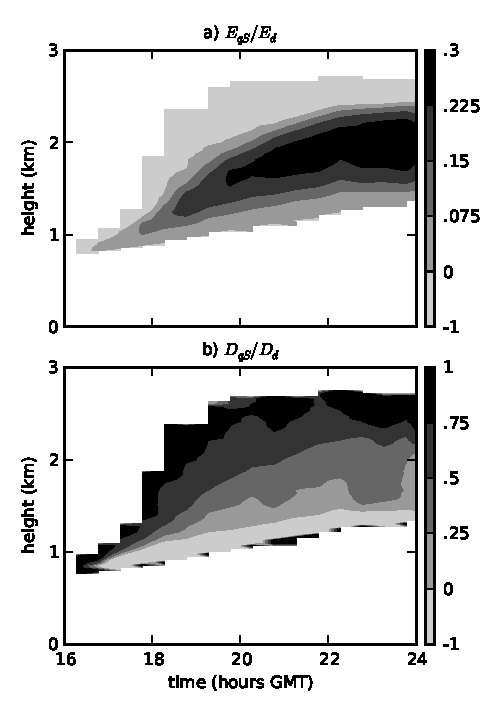
\includegraphics[width=19pc]{./figures/entrainment_ratio_variability}\\
  \caption{Variability of the ratio of the Siebesma tracer budget a) entrainment
  and b) detrainment values to the directly calculated values over the duration
  of the ARM model run.}
  \label{fig:entrainment_ratio_variability}
\end{figure}

\begin{figure}[t]
  \noindent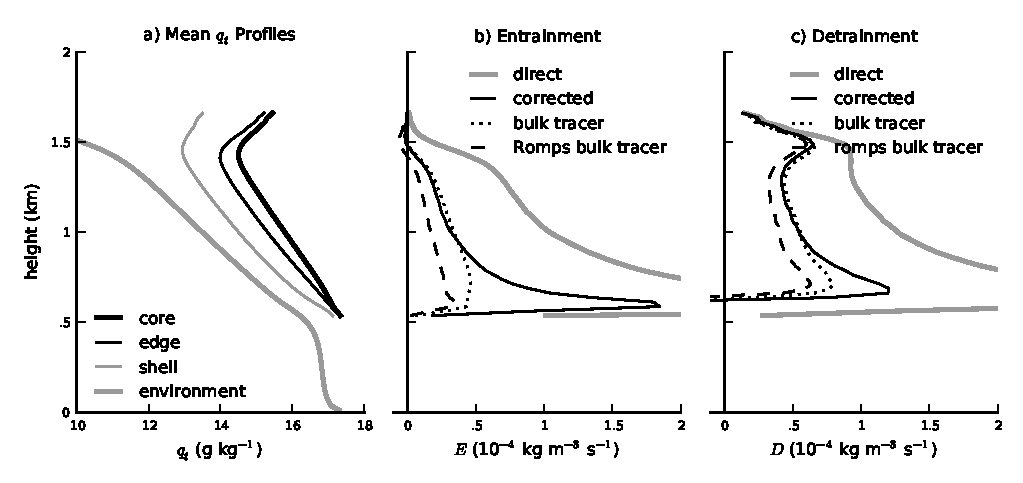
\includegraphics[width=39pc,angle=0]{./figures/shell_correction}\\
  \caption{Result of transforming direct entrainment values into equivalent 
  tracer budget values using mean cloud core shell and edge properties.  
  a) Mean profiles of the total specific humidity in the cloud core (thick 
  black line), cloud core edge (thin black line), cloud core shell (thin 
  grey line), and cloud core environment (thick grey line).  These $q_t$ 
  values are used to transform directly calculated values of (grey line) 
  b) entrainment and c) detrainment into equivalent bulk tracer budget 
  values (black line).  The Siebesma tracer budget entrainment and detrainment
  are shown for comparison (dotted lines).}
  \label{fig:Shell_correction}
\end{figure}

\begin{figure}[t]
  \noindent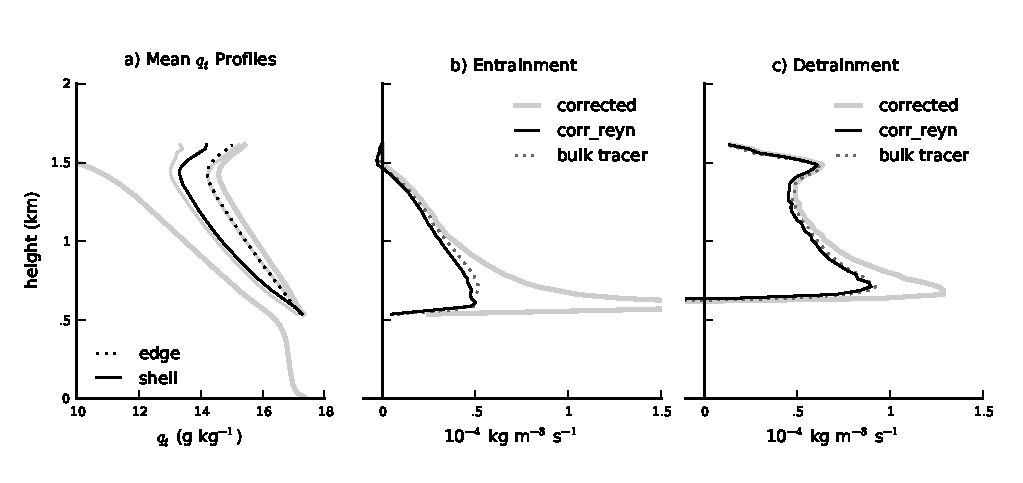
\includegraphics[width=39pc,angle=0]{./figures/reynolds_correction}\\
  \caption{Result of transforming direct entrainment values into equivalent 
  bulk tracer budget values using effective $q_t$ entrainment and detrainment 
  values.  a) Mean profiles of the effective total specific humidity values being
  entrained ($q_{entrain}$, black line), and detrained ($q_{detrain}$ dotted
  line), overlaid on the mean total specific humidity values of the core, edge, 
  shell and environment.  These $q_t$ values are used to transform directly 
  calculated values of (grey line) b) entrainment and c) detrainment into 
  equivalent bulk tracer budget values (black line).  The Siebesma tracer 
  budget entrainment and detrainment are shown for comparison (dotted lines).}
  \label{fig:Reynolds_correction}
\end{figure}

\begin{figure}[t]
  \noindent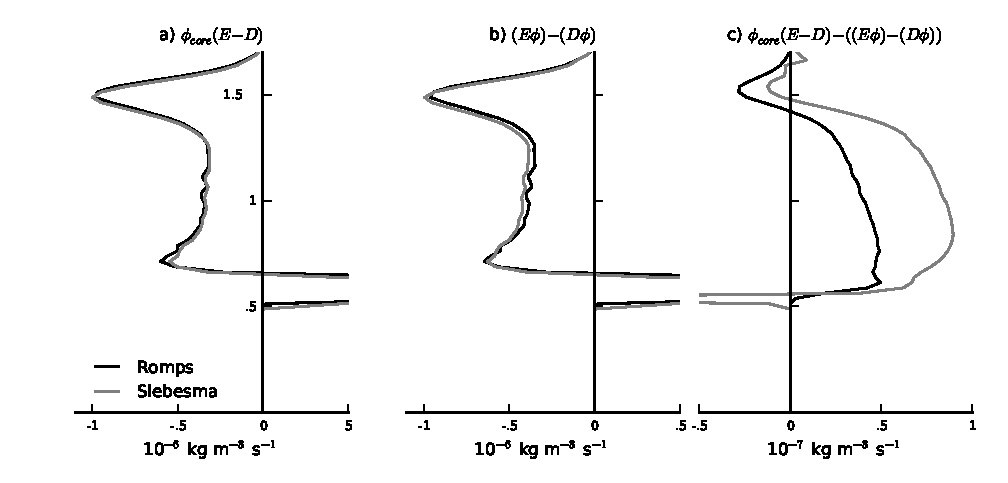
\includegraphics[width=39pc]{./figures/numerical_error}\\
  \caption{Size of a) $q_{core}(E-D)$, b) $Eq_t-Dq_t$ and c) the resulting 
  cloud core vertical advection and time tendency specific humidity budget 
  $q_{core}(E-D) - (Eq_t-Dq_t)$ for the direct entrainment/detrainment 
  (black lines), the direct entrainment/detrainment without time averaging 
  (grey lines), and the Siebesma tracer budget entrainment/detrainment 
  (dotted lines).}
  \label{fig:numerical_error}
\end{figure}

\begin{figure}[t]
  \noindent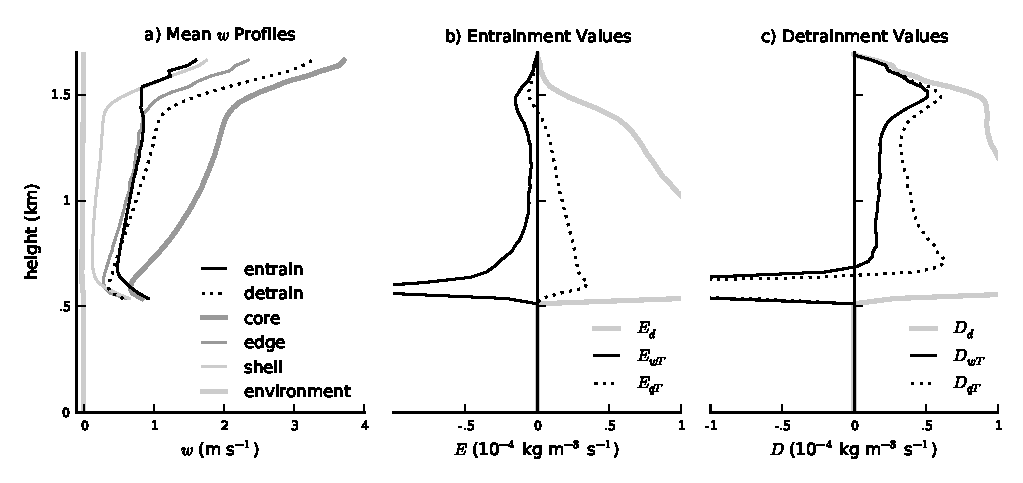
\includegraphics[width=39pc]{./figures/reynolds_correction_w}
  \caption{Result of transforming direct entrainment values into equivalent 
  bulk tracer budget values using effective $w$ entrainment and detrainment 
  values.  a) Mean profiles of the effective $w$ values being entrained 
  (black line), and detrained (dotted line), overlaid on the mean $w$ values 
  of the core, edge, shell and environment.  These $w$ values are used to
  transform directly calculated values of (grey line) b) entrainment and 
  c) detrainment into equivalent bulk tracer budget values (black line).  The  
  entrainment and detrainment values tranformed using $q_t$ are shown for
  comparison (dotted lines).}
  \label{fig:Reynolds_correction_w}
\end{figure}

\begin{figure}[t]
  \noindent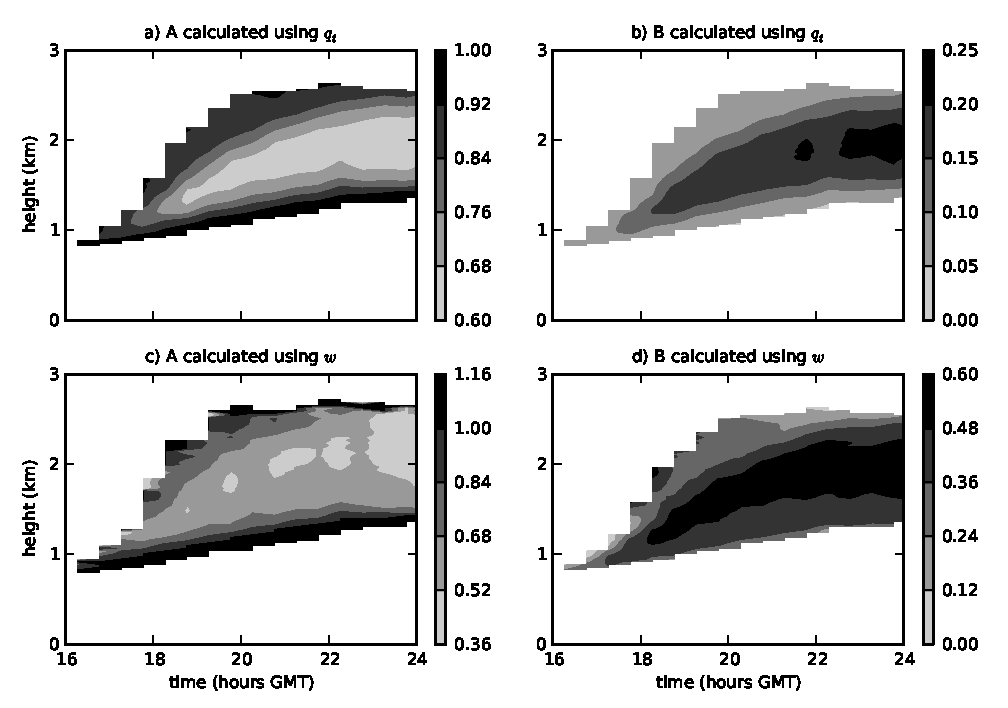
\includegraphics[width=39pc]{./figures/shell_variability}
  \caption{Variation in a) $(q_{entrain} - q_{env})/(q_{core} - q_{env})$,  
  b) $(q_{core} - q_{detrain})/(q_{core} - q_{env})$,  
  c) $(w_{entrain} - w_{env})/(w_{core} - w_{env})$, and 
  d) $(w_{core} - q_{detrain})/(w_{core} - w_{env})$ over the duration of the 
  ARM model run.
  }
  \label{fig:shell_variability}
\end{figure}

\begin{figure}[t]
  \noindent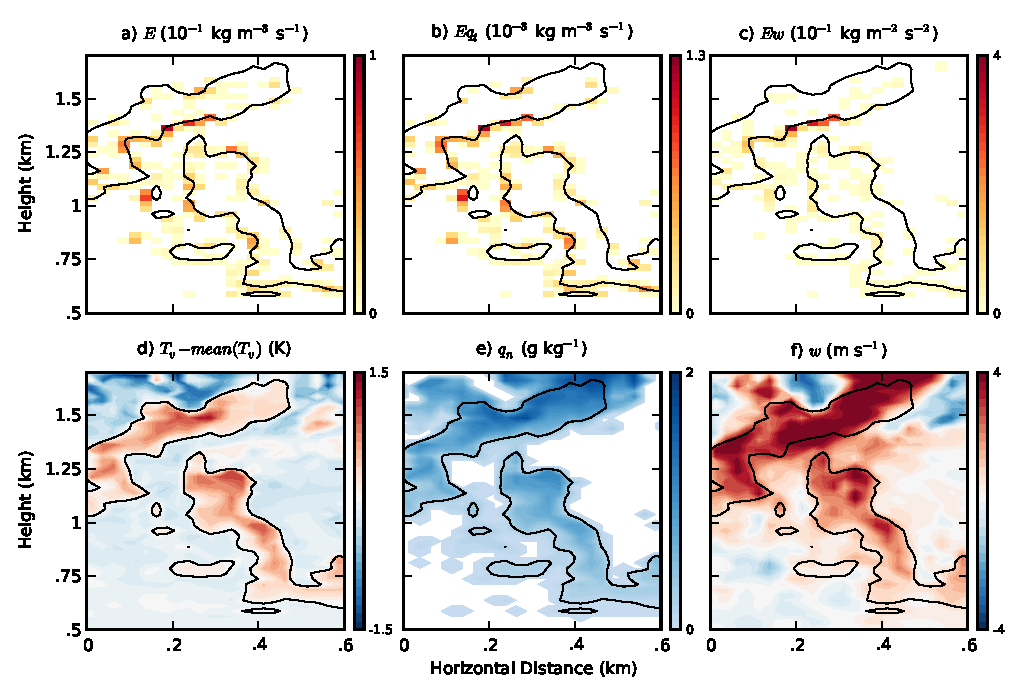
\includegraphics[width=39pc]{./figures/w_entrainment_example}
  \caption{Instantaneous vertical cross-section of directly calculated cloud 
  core mass entrainment (a), humidity entrainment (b), vertical velocity
  entrainment (c), buoyancy (d), condensed liquid water (e), and vertical
  velocity (f) of a single model cloud, illustrating the strong correlation
  between vertical velocity and entrainment.  Black lines indicate the edge of
  the cloud core in each figure.}
  \label{fig:w_entrainment_example}
\end{figure}

\end{document}
